\chapter{Guía Básica de Implementación kernel Linux OpenRISC} \label{app:apendice5}

\section{Descarga del código fuente del proyecto}

Inicialmente se deben descargar los fuentes de la sistema operativo desde el repositorio Git mediante:

\begin{lstlisting}[breaklines]
 usuario@usuario-desktop:~/\$ git clone git://git.openrisc.net/jonas/linux
\end{lstlisting}


\section{Configuración de variables de entorno}

Debe establecer la variable entorno CROSS\_COMPILE en el shell antes de iniciar la construcción del kernel Linux. Debe agregarse la siguiente línea al archivo .bashrc.

\begin{lstlisting}[breaklines]
export CROSS \_COMPILE=or32-elf-
\end{lstlisting}

Es necesario que se reconfiguren las variables mediante:
\begin{lstlisting}[breaklines]
 usuario@usuario-desktop:~/$ source ~/.bashrc
\end{lstlisting}

\section{Construcción del sistema configuración básica}

Tenga en cuenta que hay un binario pre-configurado de BusyBox. Ejecute los siguientes comandos para construir el kernel:


\begin{lstlisting}[breaklines]
usuario@usuario-desktop:~/<directorio de linux>/$ defconfig
usuario@usuario-desktop:~/<directorio de linux>/$ make
\end{lstlisting}

El archivo vmlinux ELF se convierte y se copia en el archivo vmlinux.bin al finalizar el make

\section{Ejecución del kernel en el simulador}

Utilice el siguiente comando para ejecutar el kernel de Linux en el simulador de la arquitectura OpenRISC (or1ksim): 

\begin{lstlisting}[breaklines]
usuario@usuario-desktop:~/<directorio de linux>/$or32-elf-sim -f arch/openrisc/or1ksim.cfg vmlinux
\end{lstlisting}
 
\subsection{Cambio de la configuración del UART}

La primera vez que ejecute el simulador se tiene que cambiar la configuración del UART en el archivo or1ksim  config. Agregar un terminal xterm para utilizar como dispositivo de entrada/salida.

\begin{lstlisting}[breaklines]
section uart
	enabled = 1
	baseaddr = 0x90000000
	irq = 2
	/* channel = "file:uart0.rx,uart0.tx" */
	/* channel = "tcp:10084" */
	channel = "xterm:"
	jitter = -1
	16550 = 1
end

\end{lstlisting}

\newpage
\section{Instalación sobre la placa}
La siguente guía se utiliza para la placa de desarrollo S3ADSP1800A para la configuración, compilación y descarga del Kernel.

	\subsection{Archivo de configuración para el kernel de linux}
Linux representa al hardware como device tree en un archivo .dts ~\ref{lst:dts}

\begin{lstlisting}[frame=single,caption={Xilinxs3a.dts},label={lst:dts}]

/dts-v1/;
/{
	compatible = " S3ADSP1800A";
	#address-cells =<1>;
	#size-cells = <1>;
	interrupt - parent = <&pic>;
	
	chosen{
			bootargs ="console=uart,mmio,0x90000000,115200";
			};
	
	memory@0 {
		device_type = "memory";
		reg = <0x00000000 0x08000000>
				};
	cpus{
		#address-cells =<1>;
		#size-cells = <1>;
		cpu@0{
				compatible = "opencores, or1200-rtlsvn481";
				reg =<0>;
				clock - frequency = <25000000>;
		};
	};
	pic: pic{
			compatible = "opencores, or1k-pic";
			#interrupt-cells =<1>;
			interrupt-controller;
			}
	serial0: serial@90000000 {
			compatible = "opencores, uart16550-rtlsvn105","ns16550a";
			#interrupt-cells =<2>;
			clock - frequency = <25000000>;
			};
	enet0: ethoc@92000000 {
			compatible = "opencores, ethmac-rtlsvn338";
			reg =<0x92000000 0x100>;
			#interrupt-cells =<4>;
			};
	 \end{lstlisting}

El archivo creado para la placa de desarrollo lo colocamos en: 

\begin{lstlisting}[breaklines]
usuario@usuario-desktop:~/<directorio de linux>/$arch/openrisc/boot/dts/
\end{lstlisting}

\subsection{Configuración del Kernel}

Vamos a utilizar la herramienta menuconfig para configurar el kernel para la placa. 

\begin{lstlisting}[breaklines]
usuario@usuario-desktop:~/<directorio de linux>/$make menuconfig
\end{lstlisting}

\begin{figure}[h!]
 \begin{center}
  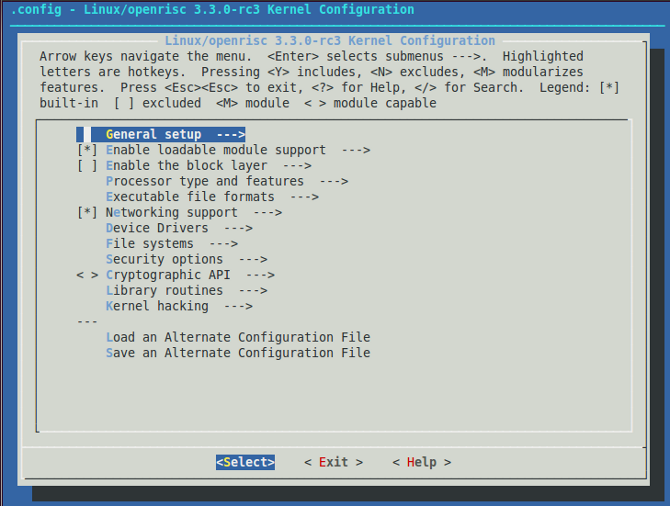
\includegraphics[width=0.5\textwidth,keepaspectratio=true]{./images/menuconf}
  \caption{Herramienta gráfica de configuración}
  %\label{fig:esquema}
 \end{center}
\end{figure}

Seleccionar el tipo de procesador, características y pulsa RETURN. 
\begin{figure}[h!]
 \begin{center}
  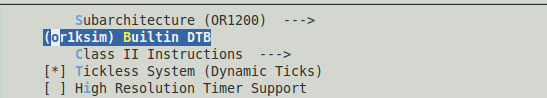
\includegraphics[width=0.5\textwidth,keepaspectratio=true]{./images/tipoprocesador}
  \caption{Herramienta gráfica de configuración}
  %\label{fig:esquema}
 \end{center}
\end{figure}
  
Luego de cambiar el simulador or1ksim a Xilinx, se guarda y se ejecuta nuevamente make.

\subsection{Generación de la imagen para ser levantada por U-boot}
\begin{lstlisting}[breaklines]
usuario@usuario-desktop:~/<directorio de linux>/$/orpsocv2/u-boot /tools/mkimage -n 'Linux for OpenRISC' -A or1k -O linux -T kernel -C none -a 0 -e 0x100 -d /opt/home/svan/OpenRISC/linux/vmlinux.bin /tftpboot/uImage
\end{lstlisting}

\subsection{Descarga de la imagen de linux}

Desde u-boot utilice el siguiente comando para descargar la imagen de Linux a la SDRAM:

\begin{lstlisting}[breaklines]
tftp uImage
\end{lstlisting}


